\section{Trajectory generation}
This section describes the transformation of a raw input image into a precise geometric path suitable for the robot's end-effector. Raw images contain significant noise and artifacts; if left unaddressed, these imperfections would propagate into the trajectory generation phase, causing the UR5e robot to execute erratic, jittery motions that increase mechanical wear and reduce drawing quality. 

\subsubsection{3.1 Noise Reduction} Raw input images often contain high-frequency noise and insignificant textures that are irrelevant to the drawing task. Before edge detection, we apply Gaussian Blur and Bilateral Filtering. This step is crucial for smoothing the input signal. By suppressing high-frequency noise while preserving structural edges, we prevent the generation of "phantom" waypoints that would cause the robot to vibrate or make unnecessary micro-movements during execution.

\subsubsection{3.2 Canny Edge Detection} We utilize the Canny algorithm to identify the topological boundaries of objects within the image. This process converts the grayscale input into a binary map where edge pixels are represented as white (255) and the background as black (0). This establishes the fundamental geometry for the robot's path planning.

\subsubsection{3.3 Addressing the "Double Line" Effect with Skeletonization} Standard edge detection often produces thick boundaries, resulting in the "Double Line Effect" where the algorithm interprets a single edge as two parallel paths. To resolve this, we apply Skeletonization, which collapses these structures into a single 1-pixel wide centerline. This eliminates redundant movements and ensures the robot traces a unique, clean path.
 \begin{figure}
     \centering
     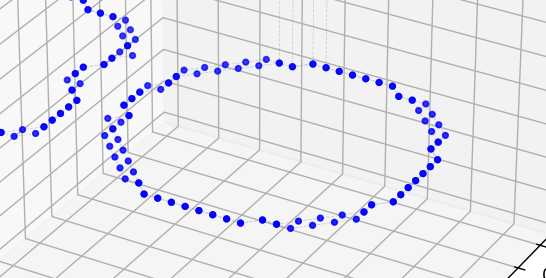
\includegraphics[width=0.5\linewidth]{FinalReport/img/doublelineeffect.png}
     \caption{Double Line Effect}
     
 \end{figure}

 \subsubsection{3.4 Path Planning and Sequence Generation}
We utilize OpenCV's \texttt{findContours} function with \texttt{CHAIN\_APPROX\_NONE} to convert the binary pixel chains into a set of vector paths. This preserves every boundary point, ensuring the robot captures high-fidelity details of the original image without simplifying curves into straight lines. The default contour order follows a scanline pattern (top-to-bottom), which causes inefficient cross-workspace travel. To minimize "air time," we implemented a Nearest Neighbor Greedy Algorithm, which uses logic to find the nearest point starting from the starting point. The algorithm iteratively selects unexplored contour lines whose starting point is closest to the robot's current end-effector position. This reordering creates a localized group of drawing paths, significantly reducing overall cycle time and unnecessary robot movements.

\subsubsection{3.5 Time-Parameterized Trajectory Generation}
Generating trajectories directly from raw contours can cause infinite acceleration at sharp corners. To address this, we impose operational limits rather than using the UR5e's theoretical maximums. To ensure precision and safety, we constrain \textbf{Drawing Velocity} ($V_{draw} \le 0.05 \, m/s$), \textbf{Travel Velocity} ($V_{travel} \le 0.25 \, m/s$), and limit acceleration ($A_{max}$) to prevent mechanical jerk.

To enforce these limits, we implemented an Iterative Time Scaling Algorithm. The system generates a trial trajectory and calculates peak velocity ($v$) and acceleration ($a$). If any value exceeds the safety limits, the segment duration ($T$) is scaled up proportionally ($a \propto 1/T^2$), and the trajectory is recomputed. This ensures the final motion is time-efficient while strictly adhering to physical constraints.

\begin{itemize}
    \item \textbf{Hybrid Trajectory Strategy and Implementation}\\
    We developed a hybrid strategy using Python (\texttt{NumPy}, \texttt{SciPy}) to handle the distinct requirements of air travel versus surface drawing.

    \item \textbf{Discrete Motion for Travel (Quintic Polynomial)}\\
    For non-drawing movements (lifting, lowering, air travel), stability is paramount. We implemented a **Quintic Polynomial** generator. This 5th-order function guarantees zero velocity and acceleration at start/stop points ($v_0=v_f=0$), ensuring a "Minimum Jerk" profile.
    \begin{equation}
        p(t) = a_0 + a_1 t + a_2 t^2 + a_3 t^3 + a_4 t^4 + a_5 t^5
    \end{equation}
    Additionally, vertical transitions (Lift/Lower) enforce a minimum duration (e.g., 0.5s) to guarantee surface clearance before lateral movement begins.

    \item\textbf{Continuous Motion for Drawing (Cubic Spline)}\\
    Stopping at every waypoint during drawing causes jitter. To achieve fluid strokes, we use **Cubic Spline Interpolation** with \textit{clamped} boundary conditions. Unlike the point-to-point Quintic method, this fits a smooth curve through the entire coordinate sequence, maintaining continuous non-zero momentum throughout the stroke while ensuring a smooth start and stop at the line's endpoints.
    \begin{equation}
        p(t) = a_0 + a_1 t + a_2 t^2 + a_3 t^3
    \end{equation}

    \item\textbf{Trajectory Output}\\
    The culmination of this pipeline is a high-resolution CSV dataset containing the full kinematic state vector $(t, x, y, z, v_x, v_y, v_z, a_x, a_y, a_z)$ for every control cycle ($dt=0.008s$). This pre-calculated trajectory serves as the direct input for the subsequent \textbf{Inverse Kinematics (IK)} solver. By providing not just position but also velocity and acceleration targets, the system enables the IK solver (or the robot controller) to compute precise joint-space commands ($\theta, \dot{\theta}, \ddot{\theta}$), ensuring the UR5e follows the generated path with high dynamic fidelity.
\end{itemize}